\documentclass[conference]{IEEEtran}
\IEEEoverridecommandlockouts
% The preceding line is only needed to identify funding in the first footnote. If that is unneeded, please comment it out.
\usepackage{cite}
\usepackage{amsmath,amssymb,amsfonts}
\usepackage{algorithmic}
\usepackage{float}
\usepackage{graphicx}
\usepackage{textcomp}
\usepackage{xcolor}
\def\BibTeX{{\rm B\kern-.05em{\sc i\kern-.025em b}\kern-.08em
    T\kern-.1667em\lower.7ex\hbox{E}\kern-.125emX}}

\DeclareGraphicsExtensions{.png,.PNG,.tiff,.tif,.jpeg,.jpg,.JPG,.JPEG,.gif}
\graphicspath{ {./images/} }

\begin{document}
\title{Software Defined Radio and it's applications
}

\author{\IEEEauthorblockN{1\textsuperscript{st} Julian Janisch}
	\IEEEauthorblockA{\textit{Mobile Computing} \\
		\textit{FH OÖ Campus Hagenberg}\\
		Hagenberg im Mühlkreis, Österreich \\
		s1710237010@students.fh-hagenberg.at}
	\and
	\IEEEauthorblockN{2\textsuperscript{nd} Alexander Kemptner}
	\IEEEauthorblockA{\textit{Mobile Computing} \\
		\textit{FH OÖ Campus Hagenberg}\\
		Hagenberg im Mühlkreis, Österreich \\
		s1710237015@students.fh-hagenberg.at}
}

\maketitle

\begin{abstract}
our abstract.\cite{Heuberger2017}
\end{abstract}

\begin{IEEEkeywords}
SDR, antenna, signal processing, ADS-B, NOAA, replay attack 
\end{IEEEkeywords}

\section{Introduction} %Julian
%Allgemein: 
% - Was ist SDR?
% - erhältliche Hardware: HackRF, SDRplay, RTL-SDR, Airspy, LimeSDR, FunCube
%   von wem kommt er? Was kostet er? Unterschiede/Möglichkeiten?

Firstly, we will explain the concept of SDR receivers (and transmitters). Afterwards, we will showcase software packages available to use with SDR receivers on the different platforms. Finally, we will present different applications using SDRs: receiving air traffic transmissions, weather satellite images and replay attacks.

\subsection{What is SDR?}
A software defined radio system is a radio transmission system that heavily relies on software instead of analog hardware~\cite[1]{Heuberger2017}.\\
In case of a transmitter, it takes data as an input (source), performs a sequence of operations via software on this data, converts it to an analog signal (with the help of an DAC) and transmits it wirelessly through its radio frequency (RF) frontend. The receiver performs the same tasks in reverse order (with an ADC), finally outputting the same data on it's sink~\cite[5-6]{wyglinski2018software}.
\begin{figure}[H]
	\centering
	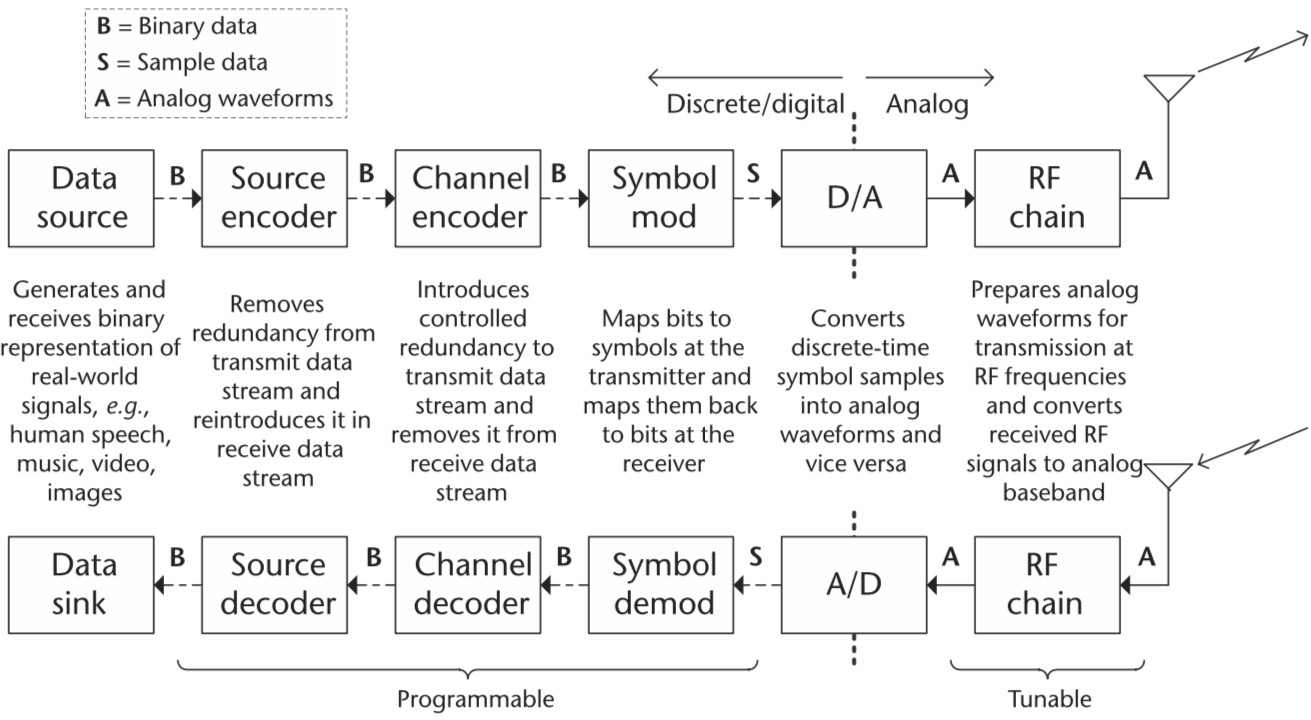
\includegraphics[width=0.5\textwidth]{forEngineers_SDR_structure}
	\caption{The structure of an SDR}
\end{figure}
In the diagram, the blocks marked as programmable can be implemented in software or programmable logic~\cite[5]{wyglinski2018software}. This makes it possible to build highly generic RF hardware that can be used for different tasks~\cite[4]{wyglinski2018software}.\\ 
The digital processing needs to be done on an IC suited for the tasks. Commonly used parts include~\cite[3]{Heuberger2017}:
\begin{itemize}
	\item FPGAs and ASICs for sample rate conversions
	\item Digital signal processors (DSPs) for expensive computations in the demodulator
	\item MCUs or CPUs for all other tasks
\end{itemize}

\subsection{Hardware}
There is various hardware on the market for software defined radio receivers and transmitters (HackRF, SDRplay, RTL-SDR, Airspy, LimeSDR, FunCube, etc.). The software defined radios we used were:
\begin{itemize}
	\item HackRF One - for data transmitting and receiving
	\item RTL-SDR - for data receivingss
	\item SDR-play - for data receiving
\end{itemize}
\bigbreak
\subsubsection{HackRF One}
Compared to the other Software Defined Radios of our list is the HackRF with a price of around 300€ the most expensive, but it has several advantages. It provides a very high operational bandwidth (from 30MHz to 6GHz) with an instantaneous bandwidth of 20MHz. (Instantaneos bandwidth = It can acquire 20MHz of RF spectrum around the chosen center frequency in real-time without a re-tuning of the oscillator) \cite[2.5]{Mishra2014} The HackRf also offers in difference to our other hardware the possibility to transmit radio signals. So it can also be used to perform replay attacks (see section \ref{replayattack}). Radio signals between 30MHz and 6GHz (e.g. Signals from remote controls of wireless sockets) can be recorded and afterwards sended again.  \\

\subsubsection{SDRplay}
\cite{sdrplay}
\\
\subsubsection{RTL-SDR}
This is the cheapest product on our list.(It did cost about 30€) The RTL-SDR is a USB-dongle which is capable of receiving radio signals  between 500kHz and 1,75GHz.  The  usage of these dongles started years ago from mass produced DVB-T TV Tuners. Because of an easy accessible chipset (RTL2832U) those tuners could be converted into wideband software defined radios (trough custom software drivers). This discovery made the access to the radio spectrum much cheaper. \cite{rtl-sdr}


\section{Software} %Alexander
%GNU Radio Companion
%CubicSDR
%GQRX
%command line tools
%SDR#
%sdrangel
% - Betriebssystem/von wem kommts/Lizenz/Funktionen/Backend
% - Was ist ein Waterfall-Diagramm?
\subsection{GNU Radio and the GNU Radio Companion}
GNU Radio is a signal processing software and software development toolkit available for Linux, OS X and (with less support available) Windows~\cite{Gnu19FAQ}\cite{Gnu19What}. It is licenced under GPLv3 or later~\cite{Gnu19FAQ}.\\
The desired signal processing steps are laid out as blocks that are connected to each other. End user applications are written using Python, while the performance-critical backend is written in C++.\\
The GNU radio companion is a GUI for GNU Radio which aids in building these blocks through drag-and-drop, comparable to Simulink~\cite{Gnu19FAQ}.\\
\begin{figure}[H]
	\centering
	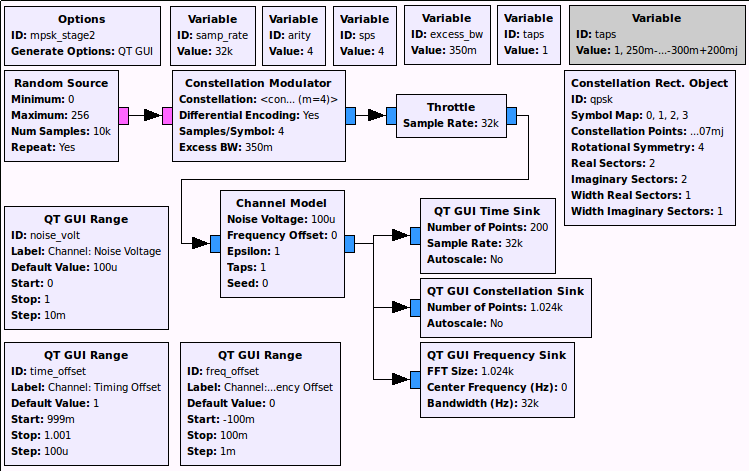
\includegraphics[width=0.5\textwidth]{gnuradio_example_flowgraph}
	\caption{An example flowgraph in GNU Radio Companion~\cite{Gnu19Example}}
\end{figure}

\subsection{GQRX}
GQRX is a graphical frontend for GNU Radio offering an FFT plot and waterfall graph, hardware abstractions for various SDRs to set frequency and other settings and multiple demodulators.\\
The received data can be digitally filtered and recorded to a file.~\cite{GQRX19Home}
\begin{figure}[H]
	\centering
	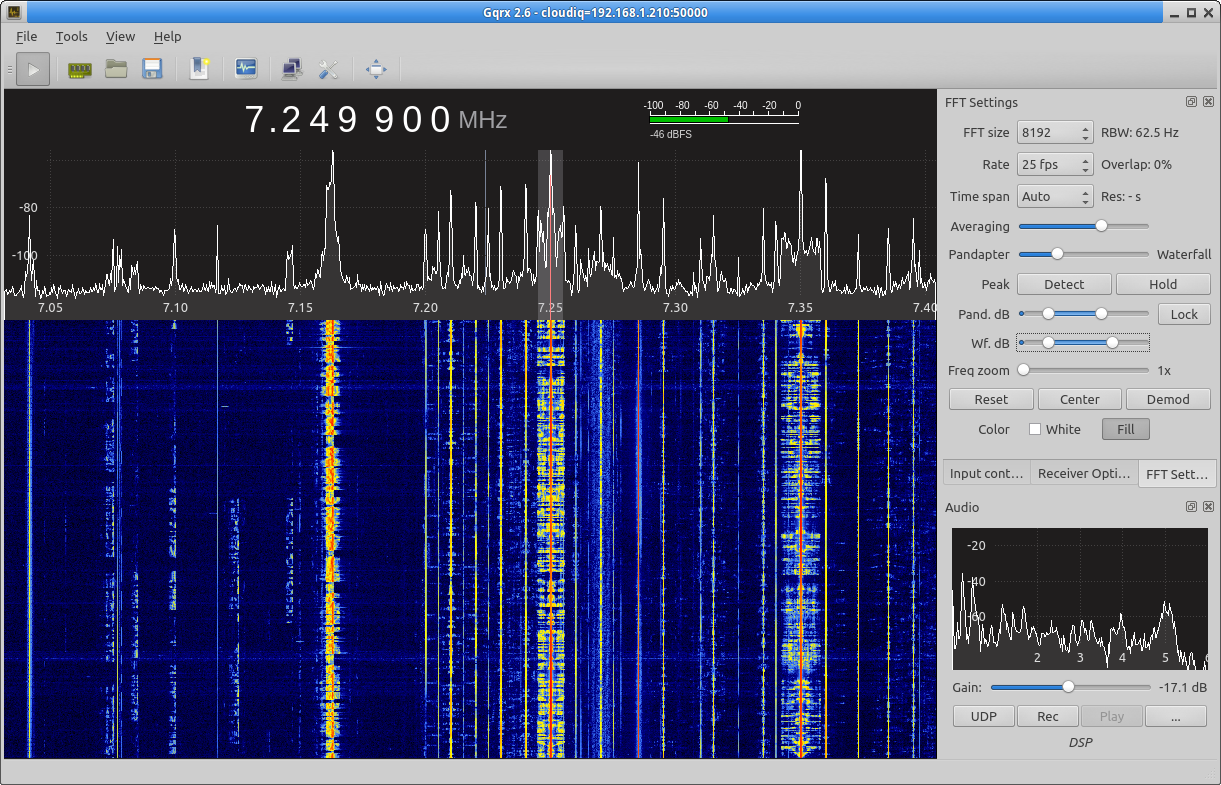
\includegraphics[width=0.5\textwidth]{gqrx_main_window}
	\caption{GQRX main window~\cite{GQRX19Home}}
\end{figure}

\subsection{SDR\#}
SDR\# (SDR sharp) is developed at Airspy for their Airspy SDRs, but can also be used with other SDRs like the RTL-SDR.\\The main software package is available for Windows only, while the "Spy Server", a program that allows streaming of the signal to clients, is available for Linux on x64/x86 and ARM (Raspberry Pi, Orange Pi).\\
The functionality can be expanded with third-party plugins~\cite{SDRsharp19Download}.

\section{ADS-B}
%Was ist ADS-B
%Wie funktioniert die Codierung?
%Welche Frequenzen gibt es? Welche Antenne wird benötigt?
%Welche Software gibt es/wie funktioniert der Workflow (hackrf_transfer/sox/dump_1090)
%Ergebnisse/Screenshots/flightradar24 Vergleich
\subsection{What is ADS-B?}


\section{NOAA SSTV} %Alexander
%Was ist NOAA
%Wie funktioniert die Codierung?
%Welche Frequenzen gibt es? Welche Antenne wird benötigt?
%Bau der Antenne (verschiedene Typen: V-Dipol, QFH, ...)
%Welche Software gibt es/wie funktioniert der Workflow
%Ergebnisse/Screenshots

\section{replay attack} %Julian
\label{replayattack}
%was ist eine replay attack?
%Beispiel Funksteckdose: Wie funktioniert die Codierung?
%wie funktioniert der workflow? HackRF + hackrf_transfer, parameter, 433 MHz Antenne

%weitere Ideen:
%Radioempfang + Codierung
%rechtliche Lage: ISM-Bänder, Amateurfunklizenz
%LTE
%ship tracking
%Antennentypen: Dipol, Yagi, Patch, Parabol, ...

\bibliography{references}
\bibliographystyle{ieeetr}

\end{document}
